\documentclass[12pt]{letter}
\usepackage{amsmath,amsfonts,amsthm,amstext,amssymb,graphicx, multicol,fancyhdr,lastpage,fullpage,framed,fancybox,enumerate,tikz,color,mathrsfs, polynom, pifont, stmaryrd}
\usepackage[margin=0.6in,headsep=3pt, headheight=15pt]{geometry}

% ----------------------------------------------------------
% Custom Definitions, Commands, Environments, etc.

% Sets of numbers
\def\R{\mathbb{R}} % The reals
\def\N{\mathbb{N}} % The naturals
\def\Z{\mathbb{Z}} % The integers
\def\Q{\mathbb{Q}} % The rationals
\def\C{\mathbb{C}} % The complex
\def\F{\mathbb{F}} % Field

% Blank space
\newcommand{\blank}[1]{\underline{\hspace{#1}}} % Blank space

% Change font colors
\newcommand{\cyan}[1]{{\color{cyan}{#1}}} % Changes font to cyan
\newcommand{\red}[1]{{\color{red}{#1}}} % Changes font to red
\newcommand{\magenta}[1]{{\color{magenta}{#1}}} % Changes font to magenta
\newcommand{\orange}[1]{{\color{orange}{#1}}} % Changes font to orange
\newcommand{\yellow}[1]{{\color{yellow}{#1}}} % Changes font to yellow
\newcommand{\violet}[1]{{\color{violet}{#1}}} % Changes font to violet
\newcommand{\green}[1]{{\color{green}{#1}}} % Changes font to green
\newcommand{\blue}[1]{{\color{blue}{#1}}} % Changes font to blue
\newcommand{\white}[1]{{\color{white}{#1}}} % Changes font to white

% Fitted inclusion symbols
\newcommand{\fp}[1]{\left({#1}\right)} % Fitted parentheses around content
\newcommand{\fb}[1]{\left[{#1}\right]} % Fitted brackets
\newcommand{\lhoi}[1]{\left({#1}\right]} % Left half-open interval
\newcommand{\rhoi}[1]{\left[{#1}\right)} % Right half-open interval
\newcommand{\set}[1]{\left\{{#1}\right\}} % Fitted braces (useful for sets)
\newcommand{\av}[1]{\left|{#1}\right|} % Fitted absolute value bars
\newcommand{\step}[1]{\left\llbracket {#1} \right\rrbracket}

% Augmented Matrix Environment
\newenvironment{amatrix}[1]{%
	\left[\begin{array}{@{}*{#1}{c}|c@{}}
	}{%
	\end{array}\right]
}

% Miscellaneous
\def\then{\Rightarrow}
\def\to{\rightarrow}
\def\d{^{\circ}}
\newcommand{\?}{\stackrel{?}{=}}
\newcommand{\cmark}{\text{ \ding{51}}}
\newcommand{\xmark}{\text{ \ding{55}}}



% Coordinate Plane (Four-Quadrant)
\def\coordplane {
	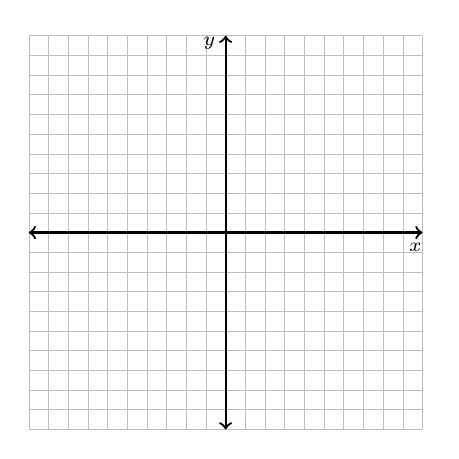
\begin{tikzpicture}        \draw[step=0.25cm,black,very thin,opacity=0.25] (-2.5cm, -2.5cm) grid (2.5cm, 2.5cm);
		\draw[<->,thick,black] (-2.5cm, 0) -- (2.5cm, 0) node[anchor=north west,pos=0.94,font=\scriptsize]{$x$};
		\draw[<->,thick,black] (0,-2.5cm) -- (0, 2.5cm) node[anchor=south east,font=\scriptsize,pos=0.94]{$y$};
	\end{tikzpicture}
}

% Coordinate Plane (One-Quadrant)
\def\onequad {
	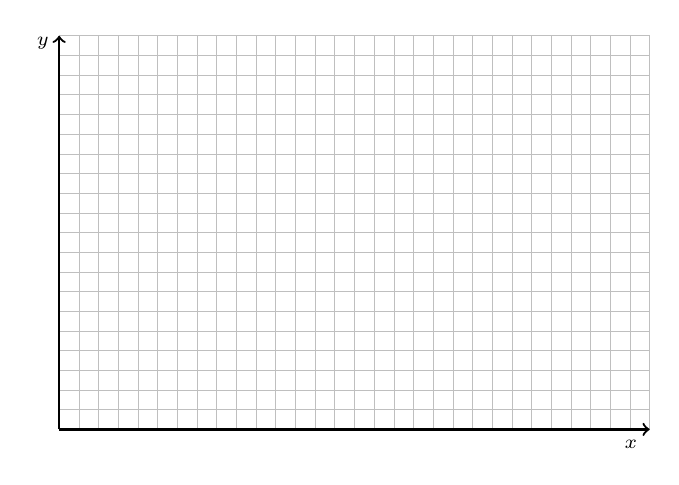
\begin{tikzpicture}
		\draw[step=0.25cm, black, very thin, opacity=0.25] (0,0) grid (7.5cm,5cm);
		\draw[->, thick, black] (0,0) -- (7.5cm, 0) node[anchor=north west,font=\scriptsize,pos=0.94]{$x$};
		\draw[->, black, thick] (0,0) -- (0,5cm) node[anchor=south east,font=\scriptsize,pos=0.94]{$y$};
	\end{tikzpicture}
}

% Counters
\newcounter{exercise}

% Exercise environment (auto-numbered)
\newenvironment{exercise}[1][]{\begin{framed}\refstepcounter{exercise}\textbf{Exercise~\theexercise:} #1}{\end{framed}}

% Book exercise environment
\newenvironment{bex}[2] {
	\begin{framed}
		\textbf{Book Exercise {#1}:} #2
	\end{framed}	
}
% ----------------------------------------------------------

% ----------------------------------------------------------
% Header and Footer Information
% \pagestyle{fancy}
% \fancyhf{}
% \renewcommand{\headrulewidth}{0pt}
% \rhead{Name: \blank{2in}}
% \lhead{@}
% \rfoot{Page \thepage \, of \,\pageref{LastPage}}
% ----------------------------------------------------------
\author{Jacob Ayers}

\begin{document}
	
	\begin{center}
		\textbf{MAT 130 \\ Assigned Exercises}
	\end{center}
	
	\textbf{Assignment 1} \begin{itemize} \vspace{-12pt}
		\item P.1 -- 8, 12, 20, 22, 38, 46, 56, 60, 64, 70
		\item P.2 -- 12, 16, 20, 26, 40, 42, 44, 54, 56, 62
		\item P.3 -- 18, 22, 34, 38, 42, 46, 50 , 76, 80
		\item P.4 -- 14, 22, 26, 30, 36, 50, 46, 56, 60, 74
	\end{itemize}

	\textbf{Assignment 2} \begin{itemize} \vspace{-12pt}
		\item P.5 -- 10, 14, 28, 34, 36, 52, 44, 50, 73
		\item P.6 -- 12, 14, 16, 24, 32, 38, 40, 44
		\item 1.1 -- 12, 18, 22, 28, 32, 38, 44, 64, 70, 74
		\item 1.2 -- 24, 28, 34, 48, 52, 62, 68, 70
	\end{itemize}

	\textbf{Assignment 3} \begin{itemize} \vspace{-12pt}
		\item 1.3 -- 32, 38, 44, 46, 50, 62, 68, 70
		\item 1.4 -- 10, 14, 24, 30, 78, 92, 106, 112
		\item 1.5 -- 14, 24, 28, 32, 34, 48, 50, 70, 76
		\item 1.6 -- 6, 14, 18, 20, 38, 48, 58, 100, 102
	\end{itemize}

	\textbf{Assignment 4} \begin{itemize} \vspace{-12pt}
		\item 1.7 -- 8, 22, 34, 42, 70, 90, 92, 96, 102
		\item 1.8 -- 8, 22, 26, 36, 40, 58, 68, 74, 78
		\item 2.1 -- 14, 18, 24, 30, 38, 66, 72, 74, 96, 98(abc)
		\item 2.2 -- 8, 10, 20, 26, 30, 42, 46, 66
	\end{itemize}

	\textbf{Assignment 5} \begin{itemize} \vspace{-12pt}
		\item 2.3 -- 12, 16, 22, 30, 36, 40, 52, 72, 80
		\item 2.4 -- 18, 24, 28, 30
		\item 2.5 -- 10(abde), 12, 14, 16, 18, 20, 44, 46
		\item 2.6 -- 8, 12, 14, 22, 30, 32, 48, 58
		\item 2.7 -- 16, 19, 22, 26, 36, 42, 44, 56, 58
	\end{itemize}

	\textbf{Assignment 6} \begin{itemize} \vspace{-12pt}
		\item 3.1 -- 5, 6, 7, 8, 48, 66, 68, 70, 72
		\item 3.2 -- 20, 26, 28, 42, 44, 74, 78, 90
		\item 3.3 -- 16, 22, 30, 36, 44, 52, 56, 64
	\end{itemize}

	\newpage
	
	\textbf{Assignment 7} \begin{itemize} \vspace{-12pt}
		\item 3.4 -- 16, 24, 28, 32, 34, 58, 74
		\item 3.5 -- 10, 14, 18, 40, 42, 44, 46, 54, 56, 58, 60, 64, 66, 70
		\item 4.1 -- 6, 12, 14, 18, 22, 26, 29, 30, 31, 32, 42, 44
	\end{itemize}

	\textbf{Assignment 8} \begin{itemize} \vspace{-12pt}
		\item 4.2 -- 16, 20, 24, 28, 32, 36, 50, 55, 58, 56, 88
		\item 5.1 -- 12, 18, 22, 26, 28, 35, 46, 52, 58, 60, 62, 64
	\end{itemize}

	\textbf{Assignment 9} \begin{itemize} \vspace{-12pt}
		\item 5.2 -- 10, 12, 16, 18, 24, 26, 28, 30, 32, 42, 58, 80, 83
		\item 5.3 -- 10, 12, 16, 22, 34, 36, 42, 46, 50, 62, 66, 70
	\end{itemize}

	\textbf{Assignment 10} \begin{itemize} \vspace{-12pt}
		\item 5.4 -- 22, 26, 30, 34, 38, 42, 48, 52, 56, 58, 60, 72, 82, 86
		\item 5.5 -- 30, 32, 34, 36, 38, 40, 42, 44, 58(ab)
	\end{itemize}

	\textbf{Assignment 11} \begin{itemize} \vspace{-12pt}
		\item 9.1 -- 6, 16, 18, 20, 30, 32, 34, 60, 64
		\item 9.2 -- 14, 18, 22, 26, 30, 36, 38, 40
		\item 9.3 -- 8, 12, 24, 28, 32, 38, 66
	\end{itemize}

	\textbf{Assignment 12} \begin{itemize} \vspace{-12pt}
		\item 10.1 -- 10, 14, 18, 24, 46, 48, 64, 66, 68, 76, 78, 80, 82, 84, 96(abcd)
	\end{itemize}
	
\end{document}